\documentclass[11pt,a4paper]{article}
\usepackage{fullpage, graphicx, url, enumitem, parskip}

\newlist{tip}{itemize}{1}
\setlist[tip,1]{
  leftmargin=\dimexpr1.2cm+\labelsep\relax,
  label={\smash{\raisebox{-0.6\height}{\includegraphics[width=1.5cm]{images/icons/tip.png}}}}
}

\newlist{arrow_red}{itemize}{1}
\setlist[arrow_red,1]{
  leftmargin=\dimexpr0.5cm+\labelsep\relax,
  label={\smash{\raisebox{-0.3\height}{\includegraphics[width=0.5cm]{images/icons/arrow_red.png}}}}
}

\newlist{arrow_yellow}{itemize}{1}
\setlist[arrow_yellow,1]{
  leftmargin=\dimexpr0.5cm+\labelsep\relax,
  label={\smash{\raisebox{-0.3\height}{\includegraphics[width=0.5cm]{images/icons/arrow_yellow.png}}}}
}

\newlist{arrow_blue}{itemize}{1}
\setlist[arrow_blue,1]{
  leftmargin=\dimexpr0.5cm+\labelsep\relax,
  label={\smash{\raisebox{-0.3\height}{\includegraphics[width=0.5cm]{images/icons/arrow_blue.png}}}}
}

\newlist{arrow_green}{itemize}{1}
\setlist[arrow_green,1]{
  leftmargin=\dimexpr0.5cm+\labelsep\relax,
  label={\smash{\raisebox{-0.3\height}{\includegraphics[width=0.5cm]{images/icons/arrow_green.png}}}}
}

\newlist{arrow_pink}{itemize}{1}
\setlist[arrow_pink,1]{
  leftmargin=\dimexpr0.5cm+\labelsep\relax,
  label={\smash{\raisebox{-0.3\height}{\includegraphics[width=0.5cm]{images/icons/arrow_pink.png}}}}
}

\setlength{\parindent}{0em}
\setlength{\parskip}{1em}

\title{\includegraphics[width=12cm]{images/logo.png}\\[1cm]SkySight 101: \\[0.5cm]A Glider Pilot's Beginner Guide}
\author{\\Matthew Scutter, Jon Pring}
\date{Updated: February 2019}


\begin{document}

\begin{titlepage}
\maketitle
\end{titlepage}

\tableofcontents
\pagebreak

\section{Introduction}
\subsection{What is Skysight}

SkySight is an interactive forecasting tool. It combines the latest forecast modelling technologies with an intuitive user interface, to provide high resolution forecasts and powerful flight planning tools.


\subsubsection{About the Development Team}


\subsection{How to use this manual}

This manual gives an overview of SkySight. It aims to provide detailed instructions on how to use the interactive forecasting features in the browser and mobile versions. Detailed descriptions of all the forecast parameters are available in the appendix.



\subsubsection{Updates}

The software is browser based, therefore you will always be using the latest version. Please ensure that your browser is up to date to ensure the best compatibility.

For LXNav and SeeYou SkySight users, updates are integrated within the regular device firmware and software updates, available at \url{http://gliding.lxnav.com} and \url{http://naviter.com}.

\subsubsection{Screenshots}

This manual often uses screenshots to visualise features. There are correct at the time of publication. However, there may be differences based on the device, browser or screen resolution.

\subsection{How to access SkySight}
SkySight is available to access and subscribe at

\url{http://skysight.io}

This gives access to all available regions and forecasting tools with a single subscription.

If you have forgotten your password, please use the \emph{forgotten password} link on the login page.


\subsubsection{Compatibility}
SkySight will work with all modern browsers, on all platforms. We recommend Chrome for the best compatibility. Our website is designed to work on all screen sizes, although some advanced features require larger screen sizes.

For mobile devices, SkySight is accessed via the browser and dedicated mobile website. We are focused on providing the best experience on all platforms, so we don't think an app is necessary.

\subsubsection{Naviter SeeYou PC}
SeeYou PC can connect with SkySight to provide forecast overlays on the native maps. This feature is available from SeeYou PC V8.0 onwards and can be used for task planning and post flight analysis. Please refer to the Naviter website at \url{http://naviter.com} for details of this feature.
\subsubsection{LXNav LX80xx/90xx}
SkySight forecast overlays are available to LXNAV users who use the LX80xx and LX90xx series of navigational instruments. The WiFi module must be installed and software updated to the latest version. Support for these devices can be found at \url{http://gliding.lxnav.com}
\subsection{Contacting SkySight}
\subsubsection{Product Support}
Please check the FAQ and this user manual before contacting SkySight support directly. If you have a query that is not covered by SkySight documentation, please contact support via the contact form at \url{http://skysight.io/contact}
\subsubsection{Feedback and Suggestions}
We are constantly looking to improve SkySight and always welcome any suggestions! Please send us any feedback to: 
\begin{flushleft}
\url{skysight@skysight.io}
\end{flushleft}
\section{Getting Started}
\subsection{User Interface}
\subsubsection{Desktop User Interface}
When SkySight is launched, the following interface will appear.
\begin{center}
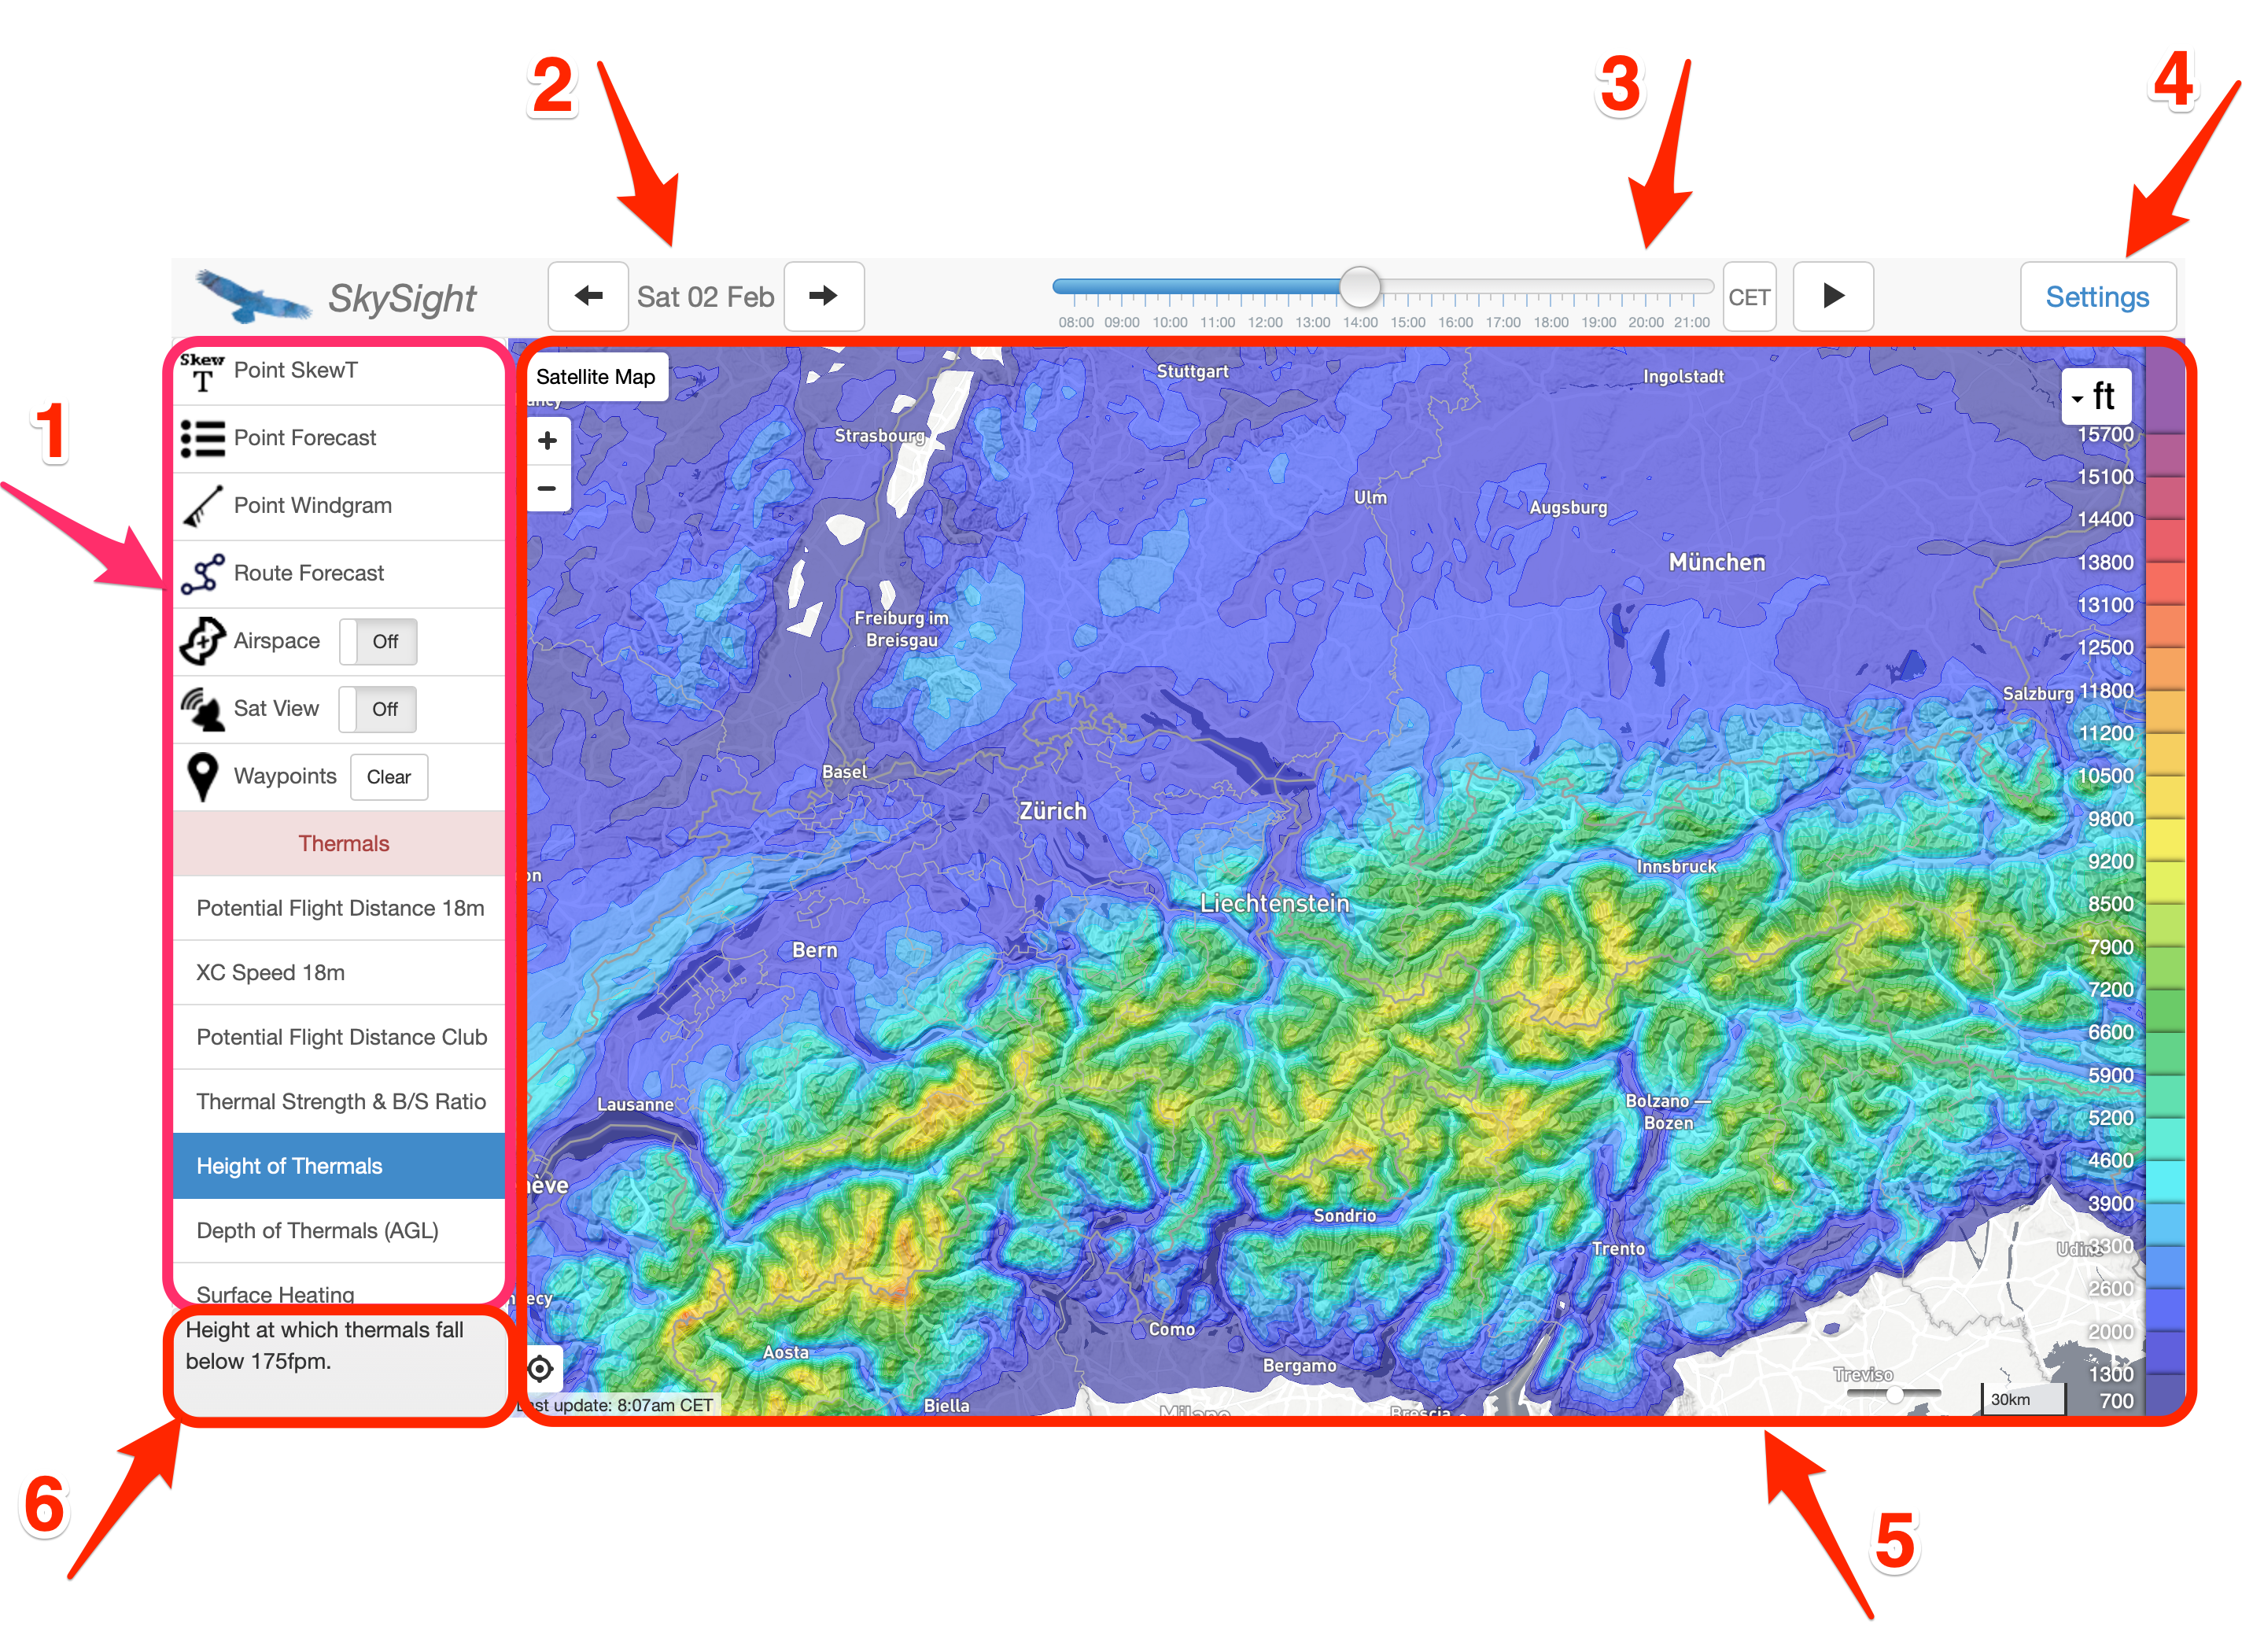
\includegraphics[width=12cm]{images/user_interface1.png}
\end{center}
\begin{enumerate}
\item \textbf{Selection Bar} -- Use this to select the interactive tools or forecast parameters.
\item \textbf{Date}  -- Use \includegraphics[height=9pt]{images/icons/previous.png} and \includegraphics[height=9pt]{images/icons/next.png}  to scroll through to the desired day. Most forecast parameters are available up to 5 days in advance. A limited duration of historic forecasts are also available.
\item \textbf{Time of Day and Time Zone} -- The slider alters the time of day. The forecast can be animated using the \includegraphics[height=9pt]{images/icons/play.png} button. There is also the option to change the time zone.
\item \textbf{Settings} -- This menu is used to change region, view account settings or log out.
\item \textbf{Map View} -- The map displays the forecast parameters overlaid on to the map in an easy to read colour scale. The map navigation features are detailed in \ref{subsec:mapnav} on page \pageref{subsec:mapnav}.
\item \textbf{Parameter Description} -- This gives a description of the forecast parameter currently selected.
\end{enumerate}
\subsubsection{Mobile User Interface}
On mobile platforms, the user interface is optimised for mobile screen sizes. The primary functionality is available, however some advanced features may not be available in mobile view.
\begin{center}
\includegraphics[height=8cm]{images/mobile_interface1.png}
\end{center}
\begin{enumerate}
\item \textbf{Selection Menu} -- Press this to access the day selection, interactive tools and forecast parameters.
\item \textbf{Time Slider} -- This slider is used to change the time of day. The time zone setting can be accessed via "desktop view" on the mobile browser.
\item \textbf{Date and Time View} -- The current day and time are visible here.
\item \textbf{Settings} -- Use this to change the region and view account settings.
\item \textbf{Scale Units} -- Press this to cycle between metric and imperial units on the map scale.
\item \textbf{GPS Location} -- This button will enable current location on the map using the device geo-location method (GPS, WiFi or GPRS).
\end{enumerate}

\begin{tip}
\item By enabling \emph{desktop view} on mobile browsers, it is possible to access all advanced features available on the desktop version.
\end{tip}
\subsection{Map Navigation} \label{subsec:mapnav}
The map section of the screen is the primary area to view forecasts. It is similar on both desktop and mobile versions. The map should update automatically once a different forecast parameter is selected or the time of day is changed.

\subsubsection{Map Zoom and Navigation}
Navigating the map should be familiar for most users. Click and drag to pan the map. 

The scale for the current zoom level is displayed in the bottom left of the map. Desktop users can scroll to zoom. Touch screen users should ``pinch" to zoom. Alternatively, use the - and + symbols on either mobile and desktop devices.
\begin{center}
\includegraphics[width=4cm]{images/map_zoom.png}
\end{center}
Satellite map view can be toggled using the ``Satellite" button in the top left. This will display a high resolution aerial photography of the map.

\subsubsection{Forecast Updates}
There are multiple forecast model runs throughout the day.
\begin{center}
\includegraphics[width=4cm]{images/last_update.png}
\end{center}
The latest forecast run time is displayed in the bottom left of the map. This is applicable to the current forecast parameter displayed on screen. This is only visible on desktop devices.

\subsubsection{Colour Scale}
On the right of the map, the colour scale is visible. The units can be cycled between metric and imperial by clicking on the unit in the top right. This colour scale will change the range automatically based on the viewing area and forecast values for that day.

\subsubsection{Colour Transparency for Colour-Blind Users}\label{subsec:colorblind}
\begin{center}
\includegraphics[width=6cm]{images/map_color1.png}
\includegraphics[width=6cm]{images/map_color2.png}
\end{center}


For colour-blind users, we have added an additional feature which changes the transparency of the forecast overlay. This helps to increase the vibrancy and contrast of the forecast. To change the transparency, move the slider at the bottom right of the map view.

\subsubsection{Exact Forecast Value}
\begin{center}
\includegraphics[width=4cm]{images/exact_value.png}
\end{center}

When a forecast parameter is selected, right-clicking on the map will display the exact forecast value. In combination with the colour map, this can be used to build up a more detailed overview of the forecast.

In mobile view, hold-press for 2 seconds on the point to use this feature.

\begin{tip}
\item This point will remain on the map until it is closed by the x. Change the time of day to see how the day develops over a specific point.
\end{tip}

\subsubsection{Airspace View}
Airspace can be displayed on the map using the \includegraphics[height=15pt]{images/icons/airspace.png} Airspace toggle. This should be considered indicative and pilots should always check local charts and NOTAMs prior to flight.
\begin{center}
\includegraphics[width=8cm]{images/airspace.png}
\end{center}

\subsubsection{Satellite View} \label{subsec:satview}
Recent satellite imagery can be toggled using \includegraphics[height=15pt]{images/icons/sat.png} Sat View. This will display up-to-date satellite imagery of cloud cover over the map, and hide the current data on the map. This is available for past and present time of day.



\begin{tip}
\item By selecting the Forecast Satellite Imagery parameter and toggling the Sat View, the forecast can be compared to the actual satellite images.
\end{tip}

\subsubsection{Nothing displayed on the map?}
If there is nothing displayed on the map, it may be for one of the following reasons.
\begin{itemize}
\item The date is out of forecast range. Please select a day closer to today's date.
\item A different region is selected. Check that the correct region for the current map view is selected in the settings menu.
\item The parameter type is out of forecast range. Some parameters are only forecast a limited number of days ahead, due to being unreliable or too resource intensive beyond a few days.
\item The overlay transparency may be set to zero. Check the Colour Transparency section \ref{subsec:colorblind} on page \pageref{subsec:colorblind} for how to adjust this.
\item The satellite view option may be turned on. Check the Satellite View section \ref {subsec:satview} on page \pageref{subsec:satview} for how to turn this off.
\item Sometimes the data set may be large and hence be slow to load on a poor internet connection. Please be patient to allow for the data to download.
\end{itemize}

\section{Interactive Tools}
SkySight includes a number of interactive tools designed to aid forecasting and route planning. This section details the basics on how to use these tools.
\subsection{Point Skew-T}
This feature displays a Skew-T log-P diagram for any point on the map at any time of day.
\begin{center}
\includegraphics[width=12cm]{images/skew-t.png}
\end{center}
\begin{arrow_red}
\item \textbf{Temperature Curve} The forecast actual temperature changing with height.
\end{arrow_red}
\begin{arrow_green}
\item \textbf{Dewpoint Curve} The forecast dewpoint temperature changing with height.
\end{arrow_green}
\begin{arrow_blue}
\item \textbf{Wind Strength} The forecast wind strength changing with height. Wind barbs are also shown.
\end{arrow_blue}
\begin{arrow_pink}
\item \textbf{Virtual Parcel} A simulated hot air parcel rising through the boundary layer. Used to predict storm development potential.
\end{arrow_pink}
To use the Skew-T tool:
\begin{enumerate}
\item Select the \includegraphics[height=15pt]{images/icons/skew-t.png} tool from the selection menu.
\item Click on the map to select the desired point for the Skew-T forecast.
\item Change the time on the top slider to see how the forecast develops over the day.
\item Move the mouse over the chart to see numerical temperature and wind for a given height.
\item The Skew-T forecast can be closed by clicking on the \includegraphics[height=11pt]{images/icons/exit.png} in the top right of the screen.
\end{enumerate}
\begin{tip}
\item The Skew-T plot is useful for validating understanding of the forecast, and showing the moisture levels in upper air-masses to help predict over-development and cloud cover.
\end{tip}
\subsection{Point Forecast}
The point forecast tool makes it easy for the development of the conditions over the whole day to be summarised quickly. Cloud cover, thermal activity and temperatures are both visualised and displayed as values.


To use the point forecast:
\begin{enumerate}
\item Select the \includegraphics[height=15pt]{images/icons/point_forecast.png} Point Forecast tool so that it is highlighted in the selection menu.
\item Click a point on the map to display the point forecast for that location.
\item Scroll down to view all the parameters.
\item The point can be moved by dragging the blue pointer on the map to the left. On small screens and mobile versions, the map will not be displayed. Close the point forecast and re-select a new location to move the point.
\item Close the point forecast by clicking on the \includegraphics[height=11pt]{images/icons/exit.png}.
\end{enumerate}
\begin{center}
\includegraphics[width=12cm]{images/point_forecast.png}
\end{center}
The cloud cover is visualised in the top rows with a colour gradient. Blue represents clear weather, whites are thin cloud, and darker greys indicate thick cloud.

Cumulus depth is represented on the convective graph with a dark grey shaded area above the condensation line. Where there is no dark grey shading, this suggests blue thermals.

\subsection{Point Windgram}
The windgram shows the development in the lapse rate, temperature, relative humidity and wind throughout the day and with height at a point. This feature is useful to visualise inversion levels, moisture layers and wind shear.
\begin{center}
\includegraphics[width=6cm]{images/windgram_lapse.png}
\includegraphics[width=6cm]{images/windgram_temp.png}\\
\includegraphics[width=6cm]{images/windgram_humid.png}
\includegraphics[width=6cm]{images/windgram_wind.png}
\end{center}

To use the windgram:
\begin{enumerate}
\item Select the \includegraphics[height=15pt]{images/icons/windgram.png} Windgram icon from the selection bar, so that it is highlighted blue.
\item Click on the map to select the desired point for the forecast.
\item Use the top drop down menu to change the parameter. Four different parameters are available including Lapse Rate, Temperature, Relative Humidity and Wind Speed.
\item The wind barbs can be shown or hidden using the check box next to the drop down menu.
\item Close the windgram by clicking on the \includegraphics[height=11pt]{images/icons/exit.png}.
\end{enumerate}

\subsection{Route Forecast}
The route forecast tool is able to estimate cross country speeds and summarise the forecast conditions over a planned task. It is a very useful tool to use during task planning and for competitions. By moving the points, it is easy to find the fastest possible tasks of the day.
\begin{center}
\includegraphics[width=12cm]{images/route.png}
\end{center}

To use this tool:
\begin{enumerate}
\item Select the \includegraphics[height=15pt]{images/icons/route.png} Route Forecast tool from the side bar, so that it is highlighted in blue.
\item Click on the map to select the desired start point. \item Click again on the map to place turn points. Repeat as necessary.
\item The route is confirmed by either returning to the start point, or by pressing `ESC' to finish the task. The optimum start times, forecast overview and task length for the route will then be displayed.
\item SkySight will automatically select the best window for the day, however it is possible to customise the task window by dragging the red start and finish times.
\item After confirming the route, it can be modified by clicking and dragging on the turn points. New turn points can be added by clicking and dragging on the small red circles on the halfway point of each leg.
\item By hovering over the route summary graph, this will show an icon on the map with the estimated location on task at that time of day.
\item The route forecast can be quit by clicking on the \includegraphics[height=15pt]{images/icons/route.png} Route Forecast icon from the side bar again.
\end{enumerate}
The route forecast tool works best with thermal tasks. The grey shaded area on the graph illustrates the depth of the cumulus. The task speeds indicated on the optimal start time dialogue are based on an 18m Ventus 2 @ 45kg/sqm flying with optimal McCready settings.
\begin{tip}
\item Check section \ref{subsec:taskplan} on page \pageref{subsec:taskplan} for tips on how to use the route forecast tool for task planning.
\end{tip}

\subsection{Wave Cross Section}
The wave cross-section tool allows wave characteristics over height to be visualised along a route. This feature is only available on desktop versions.
\begin{center}
\includegraphics[width=12cm]{images/wave_x-section.png}
\end{center}

To access this feature:
\begin{enumerate}
\item Select the \includegraphics[height=15pt]{images/icons/wave.png} Wave X-Section tool in the side bar under the Wave section.
\item Click on the map for the desired route start point.
\item Click again on the map for the end point. The cross section will then appear.
\item On large screens, the map will appear next to the cross section. Click and drag the route start and end points to move the route. Hovering over the cross section will show a vertical velocity value and the position along the route on the map.
\item The image shown will be a snapshot on a particular time. Change the time of day in the top bar to look at the development of the wave.
\item To close the cross section, click on the \includegraphics[height=11pt]{images/icons/exit.png} in the top right of the screen.
\end{enumerate}
\section{Advanced Features}
\subsection{Displaying Waypoints}
To aid task planning, SkySight includes the option to upload waypoints. These will be displayed as points on the map.  It may be necessary to zoom in to see the full waypoint names.
\begin{center}
\includegraphics[width=12cm]{images/waypoint.png}
\end{center}
To upload, click on the \includegraphics[height=15pt]{images/icons/waypoint.png} Waypoints menu and select the desired waypoint file from the device. The upload function supports SeeYou cup files only. This needs to be repeated for each individual device.

It is only possible to upload one waypoint file at a time, and the waypoints will only be visible on the device that they have been uploaded from.
\subsection{Uploading IGC files for Task Analysis}
SkySight can be used as a post-flight analysis tool. This is an especially useful tool to confirm in-flight weather observations, and to help understand their development and the interpretation of these in the SkySight forecast.

\begin{center}
\includegraphics[width=8cm]{images/igc_upload.png}
\end{center}

Click on the \includegraphics[height=15pt]{images/icons/igc.png} IGC Upload tool and select an IGC file from your device. This will overlay the trace on to the map, allowing a comparison between the forecast parameters and flown task.

Please note that to get to the correct date, this must be manually navigated to. At present, there are no features to replay the tasks in real time within SkySight, beyond the displayed trace visualisation.

\subsection{Experimental Features}
SkySight is always under development, and exciting new features are being added all the time.
\section{Getting the best out of SkySight}
\subsection{Using SkySight for Task Planning} \label{subsec:taskplan}
SkySight has a lot of useful weather information available, however interpreting it can sometimes be difficult. These basic steps below aim to get you started with using SkySight for task planning.

\begin{enumerate}
\item Determine the start of thermals. Do this by checking the thermal heights and strengths throughout the morning. Once the thermal heights and strengths are sufficient, judge this as the beginning of the day.
\item Determine the end of thermals. Use the same method as above to determine the end of the day, and therefore the length of the soaring window.
\item Check the potential flight distance. Look at this parameter over the planned task areas in combination with the soaring window worked out in (2), to calculate the re	quired task speeds.
\item Check the Cu Cloudbase throughout the day to see how convection develops. Note that positive values indicate cumulus.
\item Check the Cloud Cover  parameters to look for low, mid and high level cloud development and movement, which may affect thermal strengths.
\item Check the wind parameters, which may be an indication of streeting, wave, or convergence.
\item Having looked at all these forecasting parameters, use the route forecasting tool to plot a proposed route. The route forecast will give an estimated task speed based on different start times, and display an overview of the conditions over the task.
\item The final `gotcha' parameters to check include CAPE for storms potential, overdevelopment and rain.
\item It is always useful to validate understanding of the forecast using the Point Skew-T tool. For example, this can illustrate moisture in the airmass, changing airmasses, and vertical development.
\end{enumerate}

\subsection{Identifying Convergences}


\pagebreak
\appendix
\section{Forecast Parameters}

\subsection{Thermal}
\subsubsection{Potential Flight Distance}
\paragraph{18m}Distance an 18m Ventus 2 @ 45kg/sqm might be expected to fly, taking off at first thermals and landing at last, assuming MacCready theory in high conditions and slower in weak.
\paragraph{Club}Distance a Cirrus @ 31kg/sqm might be expected to fly, taking off at first thermals and landing at last, assuming MacCready theory in high conditions and slower in weak.
\subsubsection{Cross Country Speed}
XC Speed an 18m Ventus 2 @ 45kg/sqm might be expected to fly, in an hour, according to Macready
\subsubsection{Thermal Strength \& BS Ratio}
Strength of thermals, with increasing stipple for how broken the thermals will be (Buoyancy Shear), dense stipple possibly being unsoarable.
\subsubsection{Height of Thermals}
Height at which thermals fall below 175fpm.
\subsubsection{Depth of Thermals(AGL)}
Height above ground at which thermals fall below 175 fpm.
\subsubsection{Surface Heating}
Heat transferred into the atmosphere due to solar heating of the ground, creating thermals.
\subsection{Cloud}
\subsubsection{Cu Depth}
Difference between the top of predicted thermals and the condensation layer, increasingly positive values indicating more likely cumulus, negative values indicating unlikely cumulus.
\subsubsection{Cu Cloudbase}
In areas where cumulus is expected to form, the height of that cumulus above sea level. Grey indicates possible cloud.
\subsubsection{Overdevelopment}
Shows areas likely to overdevelop, as a percentage of 2000ft depth of overdevelopment. 0-40 indicates mild, 40-65 indicates substantial and 65+ may be unsoarable.
\subsubsection{CAPE / Storms}
Convective Available Potential Energy. Higher values indicate greater potential instability, larger updraft velocities within deep convective clouds, and greater potential for thunderstorm development.
\subsubsection{Rain}
Rain accumulated over the last half hour.
\subsubsection{Cloud Cover}
\paragraph{Low Level} Low cloud cover percentage, of any type, eg. Cu,Sc,St (1013hPa - 642hPa, 0-4,000m, 0-FL130)
\paragraph{Mid Level} Mid level cover cloud percentage, eg. Ac,As,Cb (642hPa - 350hPa, 4,000-10,000m, FL130-FL330)
\paragraph{High Level} High cloud cover percentage, eg. Ci,Cs (350hPa-150hPa, 10,000m-20,000m, FL330-FL650)
\subsubsection{Forecast Satellite View}
Cloud cover forecast intended to mimic a real satellite photo
\subsubsection{Surface Temperature}
The temperature at a height of 2m above ground level.
\subsubsection{Surface Dewpoint}
The dew point temperature at a height of 2m above ground level.
\subsection{Wind}
\subsubsection{Barbs \& Streams}
\subsubsection{Synoptic Map}
\subsubsection{Ridge Lift}
Areas of predicted ridge lift.
\subsubsection{MSL Pressure}
Atmospheric Pressure at Mean Sea Level in mBar.
\subsubsection{Surface Wind}
The speed and direction of the wind 2m above the ground.
\subsubsection{Boundary Layer Average Wind}
The speed and direction of the vector-averaged wind in the BL.
\subsubsection{Boundary Layer Top Wind}
The speed and direction of the wind at the top of the BL.
\subsubsection{Wind Shear}
Difference in wind between the top and bottom of the Boundary Layer.
\subsection{Wave}
\subsubsection{Convergence}
Maximum up/down motion within the Boundary Layer, as created by horizontal wind movement.
\subsubsection{Vertical Velocity}
Vertical velocity at specified pressure altitude, plus wind speed/direction barbs. Used for wave/convergence. Grey indicates possible cloud layers.




\end{document}
